\documentclass{article}\usepackage[]{graphicx}\usepackage[]{color}
% maxwidth is the original width if it is less than linewidth
% otherwise use linewidth (to make sure the graphics do not exceed the margin)
\makeatletter
\def\maxwidth{ %
  \ifdim\Gin@nat@width>\linewidth
    \linewidth
  \else
    \Gin@nat@width
  \fi
}
\makeatother

\definecolor{fgcolor}{rgb}{0.345, 0.345, 0.345}
\newcommand{\hlnum}[1]{\textcolor[rgb]{0.686,0.059,0.569}{#1}}%
\newcommand{\hlstr}[1]{\textcolor[rgb]{0.192,0.494,0.8}{#1}}%
\newcommand{\hlcom}[1]{\textcolor[rgb]{0.678,0.584,0.686}{\textit{#1}}}%
\newcommand{\hlopt}[1]{\textcolor[rgb]{0,0,0}{#1}}%
\newcommand{\hlstd}[1]{\textcolor[rgb]{0.345,0.345,0.345}{#1}}%
\newcommand{\hlkwa}[1]{\textcolor[rgb]{0.161,0.373,0.58}{\textbf{#1}}}%
\newcommand{\hlkwb}[1]{\textcolor[rgb]{0.69,0.353,0.396}{#1}}%
\newcommand{\hlkwc}[1]{\textcolor[rgb]{0.333,0.667,0.333}{#1}}%
\newcommand{\hlkwd}[1]{\textcolor[rgb]{0.737,0.353,0.396}{\textbf{#1}}}%
\let\hlipl\hlkwb

\usepackage{framed}
\makeatletter
\newenvironment{kframe}{%
 \def\at@end@of@kframe{}%
 \ifinner\ifhmode%
  \def\at@end@of@kframe{\end{minipage}}%
  \begin{minipage}{\columnwidth}%
 \fi\fi%
 \def\FrameCommand##1{\hskip\@totalleftmargin \hskip-\fboxsep
 \colorbox{shadecolor}{##1}\hskip-\fboxsep
     % There is no \\@totalrightmargin, so:
     \hskip-\linewidth \hskip-\@totalleftmargin \hskip\columnwidth}%
 \MakeFramed {\advance\hsize-\width
   \@totalleftmargin\z@ \linewidth\hsize
   \@setminipage}}%
 {\par\unskip\endMakeFramed%
 \at@end@of@kframe}
\makeatother

\definecolor{shadecolor}{rgb}{.97, .97, .97}
\definecolor{messagecolor}{rgb}{0, 0, 0}
\definecolor{warningcolor}{rgb}{1, 0, 1}
\definecolor{errorcolor}{rgb}{1, 0, 0}
\newenvironment{knitrout}{}{} % an empty environment to be redefined in TeX

\usepackage{alltt}

\usepackage{float}
\usepackage{hyperref}

% Set the margins on the page to not be so large
\addtolength{\oddsidemargin}{-.875in}
\addtolength{\evensidemargin}{-.875in}
\addtolength{\textwidth}{1.75in}
\addtolength{\topmargin}{-.875in}
\addtolength{\textheight}{1.75in}

% Take off page numbering
\pagenumbering{gobble}
\IfFileExists{upquote.sty}{\usepackage{upquote}}{}
\begin{document}

\title{%
6.1.2 - R: Time Series Case Study \\
\smallskip
\large Stat 5100: Dr. Bean
}
\date{}

\maketitle

\noindent Data: Weekly sales (in thousands of units) of Super Tech Videocassette Tapes over 161 weeks [see Bowerman \& O'Connell "Forecasting and Time Series: An Applied Approach", 3rd Edition, Section 10.4 Case Study. 

\noindent Goal: Want to forecast sales 25 weeks beyond end of data


\begin{knitrout}
\definecolor{shadecolor}{rgb}{0.969, 0.969, 0.969}\color{fgcolor}\begin{kframe}
\begin{alltt}
\hlkwd{library}\hlstd{(stat5100)}

\hlcom{# Manually read in the time series. Assume that the data are ordered in time}
\hlcom{# and that there are no missing weeks in the time series. }
\hlstd{sales} \hlkwb{<-} \hlkwd{c}\hlstd{(}\hlnum{45.9}\hlstd{,}  \hlnum{45.4}\hlstd{,}  \hlnum{42.8}\hlstd{,}  \hlnum{34.4}\hlstd{,} \hlnum{31.9}\hlstd{,}  \hlnum{36.6}\hlstd{,}  \hlnum{39.2}\hlstd{,}  \hlnum{41.4}\hlstd{,}
           \hlnum{40.3}\hlstd{,}  \hlnum{43.1}\hlstd{,}  \hlnum{43.2}\hlstd{,}  \hlnum{41.2}\hlstd{,} \hlnum{38.4}\hlstd{,}  \hlnum{38.3}\hlstd{,}  \hlnum{41.9}\hlstd{,}  \hlnum{37.1}\hlstd{,}
           \hlnum{34.5}\hlstd{,}  \hlnum{31.3}\hlstd{,}  \hlnum{30.2}\hlstd{,}  \hlnum{28.3}\hlstd{,} \hlnum{25.9}\hlstd{,}  \hlnum{26.6}\hlstd{,}  \hlnum{26.2}\hlstd{,}  \hlnum{29}\hlstd{,}
           \hlnum{34.8}\hlstd{,}  \hlnum{36.8}\hlstd{,}  \hlnum{37.2}\hlstd{,}  \hlnum{41.7}\hlstd{,} \hlnum{41.2}\hlstd{,}  \hlnum{40.7}\hlstd{,}  \hlnum{39.5}\hlstd{,}  \hlnum{40.4}\hlstd{,}
           \hlnum{38}\hlstd{,}    \hlnum{35.6}\hlstd{,}  \hlnum{33.9}\hlstd{,}  \hlnum{35.2}\hlstd{,} \hlnum{41.8}\hlstd{,}  \hlnum{42.4}\hlstd{,}  \hlnum{38.9}\hlstd{,}  \hlnum{42.1}\hlstd{,}
           \hlnum{41.7}\hlstd{,}  \hlnum{39.2}\hlstd{,}  \hlnum{38.5}\hlstd{,}  \hlnum{42.5}\hlstd{,} \hlnum{47.9}\hlstd{,}  \hlnum{48.6}\hlstd{,}  \hlnum{52}\hlstd{,}    \hlnum{53.5}\hlstd{,}
           \hlnum{53.5}\hlstd{,}  \hlnum{52.9}\hlstd{,}  \hlnum{53.4}\hlstd{,}  \hlnum{52.8}\hlstd{,} \hlnum{51.4}\hlstd{,}  \hlnum{52.5}\hlstd{,}  \hlnum{52.4}\hlstd{,}  \hlnum{51.5}\hlstd{,}
           \hlnum{51.7}\hlstd{,}  \hlnum{53.3}\hlstd{,}  \hlnum{55.4}\hlstd{,}  \hlnum{56.9}\hlstd{,} \hlnum{60}\hlstd{,}    \hlnum{60.8}\hlstd{,}  \hlnum{62.3}\hlstd{,}  \hlnum{62.6}\hlstd{,}
           \hlnum{63.1}\hlstd{,}  \hlnum{62.8}\hlstd{,}  \hlnum{64.7}\hlstd{,}  \hlnum{66.3}\hlstd{,} \hlnum{63}\hlstd{,}    \hlnum{65.5}\hlstd{,}  \hlnum{70.6}\hlstd{,}  \hlnum{76}\hlstd{,}
           \hlnum{80.1}\hlstd{,}  \hlnum{78.6}\hlstd{,}  \hlnum{78.3}\hlstd{,}  \hlnum{78.1}\hlstd{,} \hlnum{73.6}\hlstd{,}  \hlnum{68.8}\hlstd{,}  \hlnum{64.4}\hlstd{,}  \hlnum{62.4}\hlstd{,}
           \hlnum{61.1}\hlstd{,}  \hlnum{63.1}\hlstd{,}  \hlnum{65.3}\hlstd{,}  \hlnum{68.3}\hlstd{,} \hlnum{72.5}\hlstd{,}  \hlnum{73.2}\hlstd{,}  \hlnum{72.9}\hlstd{,}  \hlnum{70.5}\hlstd{,}
           \hlnum{69.4}\hlstd{,}  \hlnum{68.2}\hlstd{,}  \hlnum{69.3}\hlstd{,}  \hlnum{72.3}\hlstd{,} \hlnum{73.5}\hlstd{,}  \hlnum{70.3}\hlstd{,}  \hlnum{68.3}\hlstd{,}  \hlnum{64.1}\hlstd{,}
           \hlnum{62.5}\hlstd{,}  \hlnum{62.6}\hlstd{,}  \hlnum{60.4}\hlstd{,}  \hlnum{61.1}\hlstd{,} \hlnum{64.7}\hlstd{,}  \hlnum{65.1}\hlstd{,}  \hlnum{61.5}\hlstd{,}  \hlnum{64.2}\hlstd{,}
           \hlnum{67.8}\hlstd{,}  \hlnum{66.8}\hlstd{,}  \hlnum{64.1}\hlstd{,}  \hlnum{66.4}\hlstd{,} \hlnum{68}\hlstd{,}    \hlnum{71}\hlstd{,}    \hlnum{76.9}\hlstd{,}  \hlnum{84.1}\hlstd{,}
           \hlnum{85.9}\hlstd{,}  \hlnum{85.2}\hlstd{,}  \hlnum{86.2}\hlstd{,}  \hlnum{85.7}\hlstd{,} \hlnum{81.3}\hlstd{,}  \hlnum{75.9}\hlstd{,}  \hlnum{75}\hlstd{,}    \hlnum{72.5}\hlstd{,}
           \hlnum{69.6}\hlstd{,}  \hlnum{67.3}\hlstd{,}  \hlnum{69.8}\hlstd{,}  \hlnum{72.2}\hlstd{,} \hlnum{75.2}\hlstd{,}  \hlnum{77.2}\hlstd{,}  \hlnum{76.8}\hlstd{,}  \hlnum{72.4}\hlstd{,}
           \hlnum{69.4}\hlstd{,}  \hlnum{68.7}\hlstd{,}  \hlnum{65.1}\hlstd{,}  \hlnum{64.4}\hlstd{,} \hlnum{64.2}\hlstd{,}  \hlnum{63.2}\hlstd{,}  \hlnum{62.1}\hlstd{,}  \hlnum{65.8}\hlstd{,}
           \hlnum{73.7}\hlstd{,}  \hlnum{77.1}\hlstd{,}  \hlnum{76}\hlstd{,}    \hlnum{74.6}\hlstd{,} \hlnum{70.6}\hlstd{,}  \hlnum{67.5}\hlstd{,}  \hlnum{67.9}\hlstd{,}  \hlnum{68.9}\hlstd{,}
           \hlnum{67.8}\hlstd{,}  \hlnum{65.1}\hlstd{,}  \hlnum{65}\hlstd{,}    \hlnum{67.6}\hlstd{,} \hlnum{67.9}\hlstd{,}  \hlnum{66.5}\hlstd{,}  \hlnum{68.2}\hlstd{,}  \hlnum{71.7}\hlstd{,}
           \hlnum{71.3}\hlstd{,}  \hlnum{68.9}\hlstd{,}  \hlnum{70}\hlstd{,}    \hlnum{73.1}\hlstd{,} \hlnum{69.1}\hlstd{,}  \hlnum{67.3}\hlstd{,}  \hlnum{72.9}\hlstd{,}  \hlnum{78.6}\hlstd{,}  \hlnum{82.3}\hlstd{)}
\end{alltt}
\end{kframe}
\end{knitrout}


\subsection*{Look at original data and check stationarity}

\begin{knitrout}
\definecolor{shadecolor}{rgb}{0.969, 0.969, 0.969}\color{fgcolor}\begin{kframe}
\begin{alltt}
\hlcom{# Create Time Series }
\hlstd{sales_ts} \hlkwb{<-} \hlkwd{ts}\hlstd{(sales)}

\hlcom{# Sample Autocorrelation Plot (ACF) / Sample Partial Autocorrelation Plots (PACF)}
\hlkwd{par}\hlstd{(}\hlkwc{mfrow} \hlstd{=} \hlkwd{c}\hlstd{(}\hlnum{2}\hlstd{,} \hlnum{2}\hlstd{))}
\hlkwd{plot}\hlstd{(sales_ts)}
\hlkwd{points}\hlstd{(sales_ts)}
\hlkwd{acf}\hlstd{(sales_ts,} \hlkwc{lag.max} \hlstd{=} \hlnum{12}\hlstd{)}
\hlkwd{pacf}\hlstd{(sales_ts,} \hlkwc{lag.max} \hlstd{=} \hlnum{12}\hlstd{)}
\hlkwd{par}\hlstd{(}\hlkwc{mfrow} \hlstd{=} \hlkwd{c}\hlstd{(}\hlnum{1}\hlstd{,} \hlnum{1}\hlstd{))}
\end{alltt}
\end{kframe}

{\centering 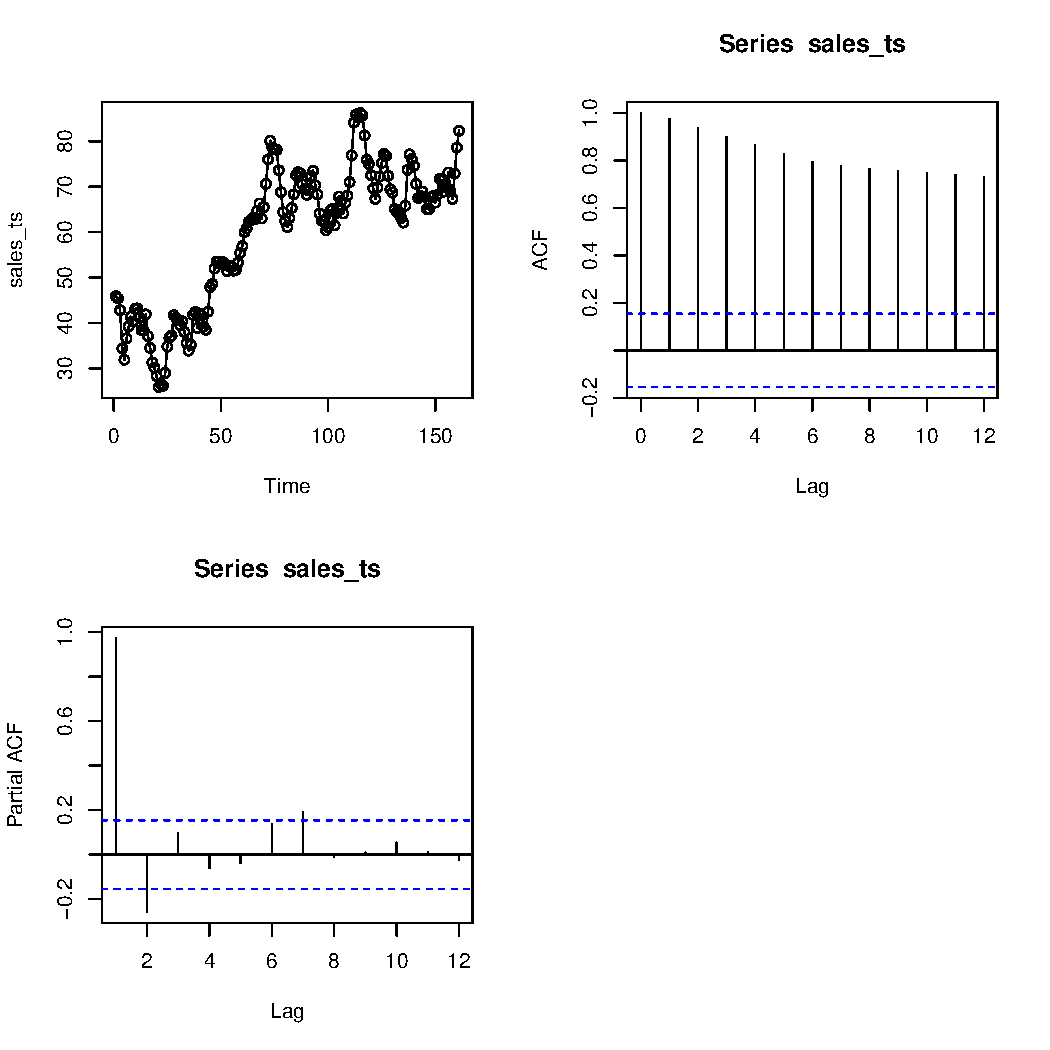
\includegraphics[width=0.9\textwidth]{figure/unnamed-chunk-2-1} 

}


\begin{kframe}\begin{alltt}
\hlcom{# Autocorrelation check for white noise}
\hlkwd{Box.test}\hlstd{(sales_ts,} \hlkwc{lag} \hlstd{=} \hlnum{6}\hlstd{,} \hlkwc{type} \hlstd{=} \hlstr{"Ljung"}\hlstd{)}
\end{alltt}
\begin{verbatim}
## 
## 	Box-Ljung test
## 
## data:  sales_ts
## X-squared = 779.33, df = 6, p-value < 2.2e-16
\end{verbatim}
\begin{alltt}
\hlkwd{Box.test}\hlstd{(sales_ts,} \hlkwc{lag} \hlstd{=} \hlnum{12}\hlstd{,} \hlkwc{type} \hlstd{=} \hlstr{"Ljung"}\hlstd{)}
\end{alltt}
\begin{verbatim}
## 
## 	Box-Ljung test
## 
## data:  sales_ts
## X-squared = 1366.7, df = 12, p-value < 2.2e-16
\end{verbatim}
\end{kframe}
\end{knitrout}

The ACF plot descends very slowly, which is evidence of nonstationarity. Also, there seems to be an obvious increase trend in sales over time. (Apparently, they haven't invented streaming services yet...)

\subsubsection*{Remove linear effect of time and recheck for stationarity.}

\begin{knitrout}
\definecolor{shadecolor}{rgb}{0.969, 0.969, 0.969}\color{fgcolor}\begin{kframe}
\begin{alltt}
\hlstd{sales_df} \hlkwb{<-} \hlkwd{data.frame}\hlstd{(}\hlkwc{sales} \hlstd{= sales,} \hlkwc{time} \hlstd{=} \hlnum{1}\hlopt{:}\hlkwd{length}\hlstd{(sales))}

\hlstd{sales_lm} \hlkwb{<-} \hlkwd{lm}\hlstd{(sales} \hlopt{~} \hlstd{time,} \hlkwc{data} \hlstd{= sales_df)}

\hlstd{resid_ts} \hlkwb{<-} \hlkwd{ts}\hlstd{(sales_lm}\hlopt{$}\hlstd{residuals)}

\hlcom{# Sample Autocorrelation Plot (ACF) / Sample Partial Autocorrelation Plots (PACF)}
\hlkwd{par}\hlstd{(}\hlkwc{mfrow} \hlstd{=} \hlkwd{c}\hlstd{(}\hlnum{2}\hlstd{,} \hlnum{2}\hlstd{))}
\hlkwd{plot}\hlstd{(resid_ts)}
\hlkwd{points}\hlstd{(resid_ts)}
\hlkwd{acf}\hlstd{(resid_ts,} \hlkwc{lag.max} \hlstd{=} \hlnum{12}\hlstd{)}
\hlkwd{pacf}\hlstd{(resid_ts,} \hlkwc{lag.max} \hlstd{=} \hlnum{12}\hlstd{)}
\hlkwd{par}\hlstd{(}\hlkwc{mfrow} \hlstd{=} \hlkwd{c}\hlstd{(}\hlnum{1}\hlstd{,} \hlnum{1}\hlstd{))}
\end{alltt}
\end{kframe}

{\centering 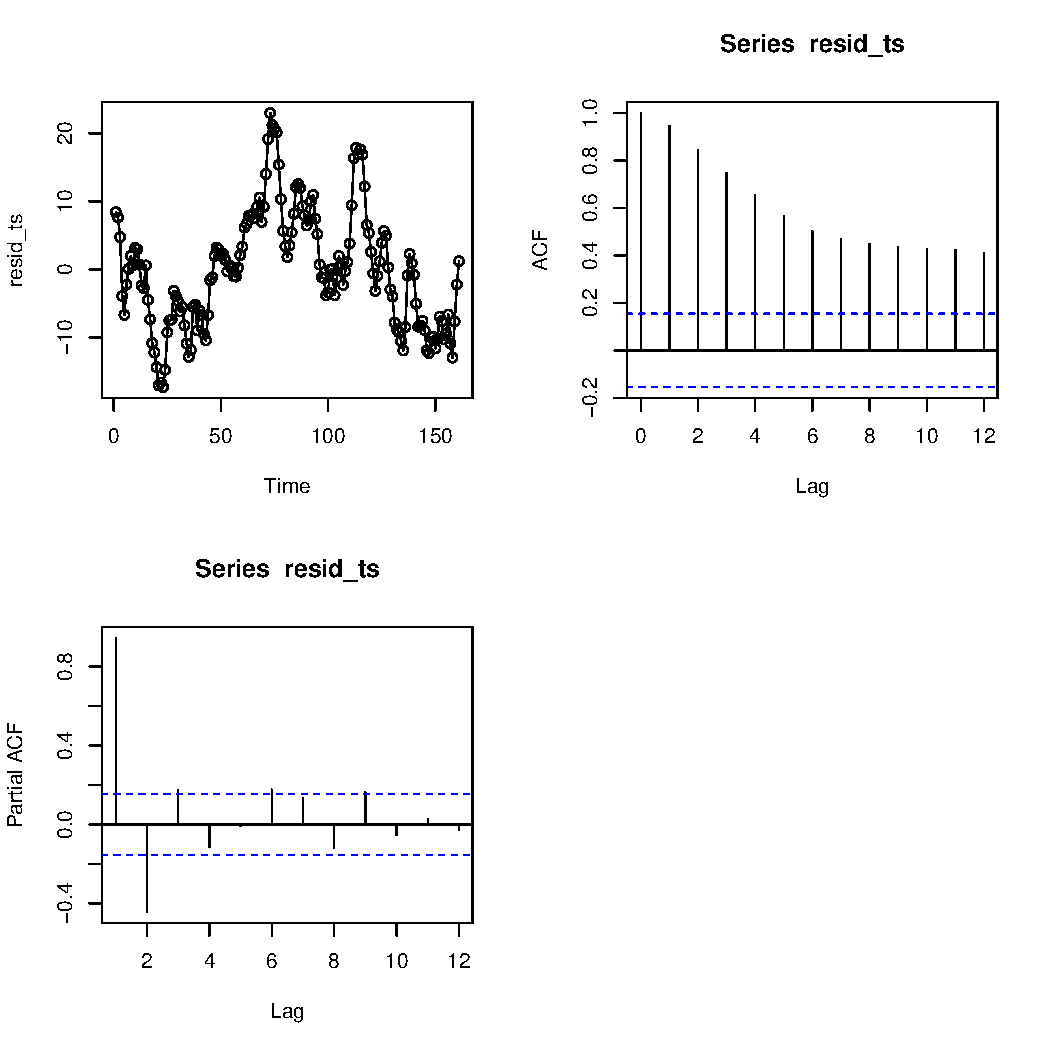
\includegraphics[width=0.6\textwidth]{figure/unnamed-chunk-3-1} 

}


\begin{kframe}\begin{alltt}
\hlcom{# Autocorrelation check for white noise}
\hlkwd{Box.test}\hlstd{(resid_ts,} \hlkwc{lag} \hlstd{=} \hlnum{6}\hlstd{,} \hlkwc{type} \hlstd{=} \hlstr{"Ljung"}\hlstd{)}
\end{alltt}
\begin{verbatim}
## 
## 	Box-Ljung test
## 
## data:  resid_ts
## X-squared = 523.89, df = 6, p-value < 2.2e-16
\end{verbatim}
\begin{alltt}
\hlkwd{Box.test}\hlstd{(resid_ts,} \hlkwc{lag} \hlstd{=} \hlnum{12}\hlstd{,} \hlkwc{type} \hlstd{=} \hlstr{"Ljung"}\hlstd{)}
\end{alltt}
\begin{verbatim}
## 
## 	Box-Ljung test
## 
## data:  resid_ts
## X-squared = 720.33, df = 12, p-value < 2.2e-16
\end{verbatim}
\end{kframe}
\end{knitrout}

ACF plot is still decreasing too slowly. It looks like this might be due to cyclic behavior in the residuals. We will try a new trend model that will remove what seems to be a two year (104 week) cycle in the residuals.

\begin{knitrout}
\definecolor{shadecolor}{rgb}{0.969, 0.969, 0.969}\color{fgcolor}\begin{kframe}
\begin{alltt}
\hlstd{sales_lm_2} \hlkwb{<-} \hlkwd{lm}\hlstd{(sales} \hlopt{~} \hlstd{time} \hlopt{+} \hlkwd{sin}\hlstd{(}\hlnum{2}\hlopt{*}\hlstd{pi}\hlopt{*}\hlstd{time}\hlopt{/}\hlnum{104}\hlstd{)} \hlopt{+} \hlkwd{cos}\hlstd{(}\hlnum{2}\hlopt{*}\hlstd{pi}\hlopt{*}\hlstd{time}\hlopt{/}\hlnum{104}\hlstd{),} \hlkwc{data} \hlstd{= sales_df)}

\hlstd{resid_ts_2} \hlkwb{<-} \hlkwd{ts}\hlstd{(sales_lm_2}\hlopt{$}\hlstd{residuals)}

\hlcom{# Sample Autocorrelation Plot (ACF) / Sample Partial Autocorrelation Plots (PACF)}
\hlkwd{par}\hlstd{(}\hlkwc{mfrow} \hlstd{=} \hlkwd{c}\hlstd{(}\hlnum{2}\hlstd{,} \hlnum{2}\hlstd{))}
\hlkwd{plot}\hlstd{(resid_ts_2)}
\hlkwd{points}\hlstd{(resid_ts_2)}
\hlkwd{acf}\hlstd{(resid_ts_2,} \hlkwc{lag.max} \hlstd{=} \hlnum{12}\hlstd{)}
\hlkwd{pacf}\hlstd{(resid_ts_2,} \hlkwc{lag.max} \hlstd{=} \hlnum{12}\hlstd{)}
\hlkwd{par}\hlstd{(}\hlkwc{mfrow} \hlstd{=} \hlkwd{c}\hlstd{(}\hlnum{1}\hlstd{,} \hlnum{1}\hlstd{))}
\end{alltt}
\end{kframe}
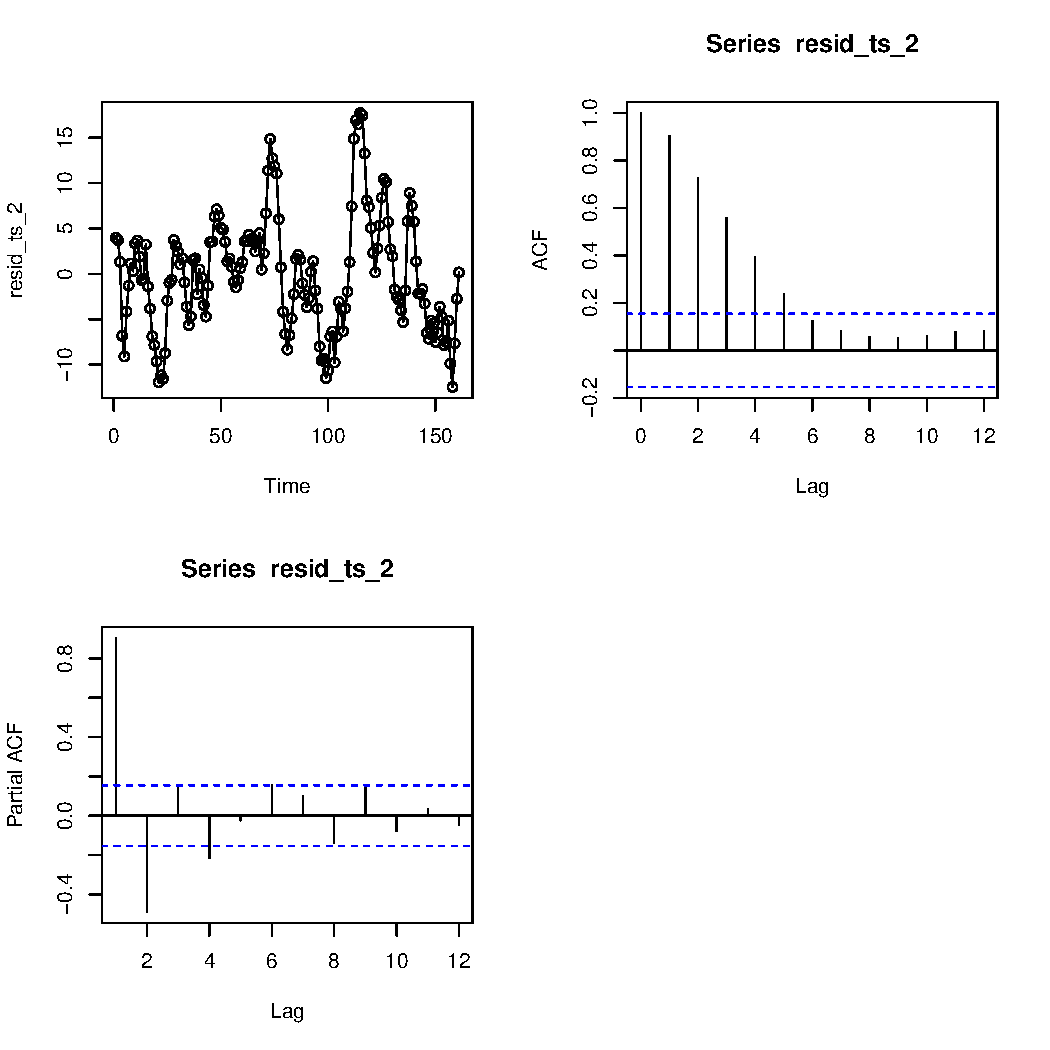
\includegraphics[width=\maxwidth]{figure/unnamed-chunk-4-1} 
\begin{kframe}\begin{alltt}
\hlcom{# Autocorrelation check for white noise}
\hlkwd{Box.test}\hlstd{(resid_ts_2,} \hlkwc{lag} \hlstd{=} \hlnum{6}\hlstd{,} \hlkwc{type} \hlstd{=} \hlstr{"Ljung"}\hlstd{)}
\end{alltt}
\begin{verbatim}
## 
## 	Box-Ljung test
## 
## data:  resid_ts_2
## X-squared = 310.25, df = 6, p-value < 2.2e-16
\end{verbatim}
\begin{alltt}
\hlkwd{Box.test}\hlstd{(resid_ts_2,} \hlkwc{lag} \hlstd{=} \hlnum{12}\hlstd{,} \hlkwc{type} \hlstd{=} \hlstr{"Ljung"}\hlstd{)}
\end{alltt}
\begin{verbatim}
## 
## 	Box-Ljung test
## 
## data:  resid_ts_2
## X-squared = 315.11, df = 12, p-value < 2.2e-16
\end{verbatim}
\end{kframe}
\end{knitrout}

This looks better, but still not a stationary process (ACF is still decreasing too slowly). We will now resort to differencing as a way to achieve stationarity. 

\begin{knitrout}
\definecolor{shadecolor}{rgb}{0.969, 0.969, 0.969}\color{fgcolor}\begin{kframe}
\begin{alltt}
\hlstd{sales_d1} \hlkwb{<-} \hlkwd{ts}\hlstd{(}\hlkwd{diff}\hlstd{(sales,} \hlkwc{lag} \hlstd{=} \hlnum{1}\hlstd{))}

\hlcom{# Sample Autocorrelation Plot (ACF) / Sample Partial Autocorrelation Plots (PACF)}
\hlkwd{par}\hlstd{(}\hlkwc{mfrow} \hlstd{=} \hlkwd{c}\hlstd{(}\hlnum{2}\hlstd{,} \hlnum{2}\hlstd{))}
\hlkwd{plot}\hlstd{(sales_d1)}
\hlkwd{points}\hlstd{(sales_d1)}
\hlkwd{acf}\hlstd{(sales_d1,} \hlkwc{lag.max} \hlstd{=} \hlnum{12}\hlstd{)}
\hlkwd{pacf}\hlstd{(sales_d1,} \hlkwc{lag.max} \hlstd{=} \hlnum{12}\hlstd{)}
\hlkwd{par}\hlstd{(}\hlkwc{mfrow} \hlstd{=} \hlkwd{c}\hlstd{(}\hlnum{1}\hlstd{,} \hlnum{1}\hlstd{))}
\end{alltt}
\end{kframe}
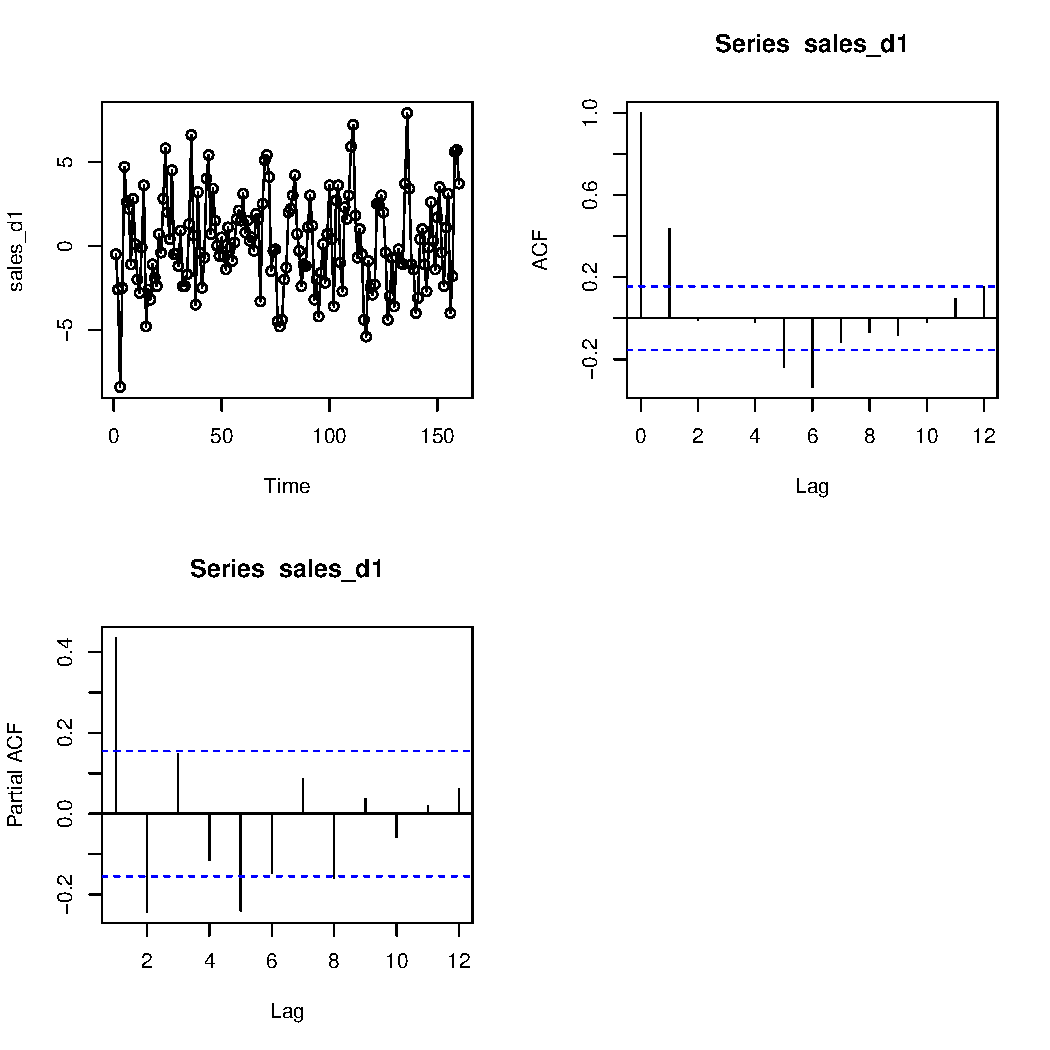
\includegraphics[width=\maxwidth]{figure/unnamed-chunk-5-1} 
\begin{kframe}\begin{alltt}
\hlcom{# Autocorrelation check for white noise}
\hlkwd{Box.test}\hlstd{(sales_d1,} \hlkwc{lag} \hlstd{=} \hlnum{6}\hlstd{,} \hlkwc{type} \hlstd{=} \hlstr{"Ljung"}\hlstd{)}
\end{alltt}
\begin{verbatim}
## 
## 	Box-Ljung test
## 
## data:  sales_d1
## X-squared = 59.37, df = 6, p-value = 6.044e-11
\end{verbatim}
\begin{alltt}
\hlkwd{Box.test}\hlstd{(sales_d1,} \hlkwc{lag} \hlstd{=} \hlnum{12}\hlstd{,} \hlkwc{type} \hlstd{=} \hlstr{"Ljung"}\hlstd{)}
\end{alltt}
\begin{verbatim}
## 
## 	Box-Ljung test
## 
## data:  sales_d1
## X-squared = 68.799, df = 12, p-value = 5.369e-10
\end{verbatim}
\end{kframe}
\end{knitrout}

The Box-Ljung test indicates significant autocorrelation and the ACF/PACF plots show no evidence of non-stationarity. As such, we can now determine which dependence structures to fit to account for the autocorrelation. 

\subsubsection*{Model 1: ARIMA(2, 1, 0)}

The ACF plot has a damped exponential/sine pattern and the PACF has spikes at 1 and 2. Based on this, we will try fitting an AR(2) structure to the first-order difference time series. 

\begin{knitrout}
\definecolor{shadecolor}{rgb}{0.969, 0.969, 0.969}\color{fgcolor}\begin{kframe}
\begin{alltt}
\hlcom{# Note that I am using the original time series, not the differenced }
\hlcom{# time series, and am including the differencing term within the arima statement. }
\hlstd{sales_arima} \hlkwb{<-} \hlstd{forecast}\hlopt{::}\hlkwd{Arima}\hlstd{(sales_ts,} \hlkwc{order} \hlstd{=} \hlkwd{c}\hlstd{(}\hlnum{2}\hlstd{,} \hlnum{1}\hlstd{,} \hlnum{0}\hlstd{),}
                               \hlkwc{include.drift} \hlstd{=} \hlnum{FALSE}\hlstd{)}
\end{alltt}


{\ttfamily\noindent\itshape\color{messagecolor}{\#\# Registered S3 method overwritten by 'quantmod':\\\#\#\ \  method\ \ \ \ \ \ \ \ \ \ \ \ from\\\#\#\ \  as.zoo.data.frame zoo}}\begin{alltt}
\hlkwd{summary}\hlstd{(sales_arima)}
\end{alltt}
\begin{verbatim}
## Series: sales_ts 
## ARIMA(2,1,0) 
## 
## Coefficients:
##          ar1      ar2
##       0.5425  -0.2393
## s.e.  0.0766   0.0775
## 
## sigma^2 estimated as 6.134:  log likelihood=-371.3
## AIC=748.6   AICc=748.75   BIC=757.83
## 
## Training set error measures:
##                     ME     RMSE     MAE       MPE     MAPE      MASE       ACF1
## Training set 0.1568165 2.453555 1.95076 0.1872017 3.635346 0.8655618 0.03509532
\end{verbatim}
\begin{alltt}
\hlstd{lmtest}\hlopt{::}\hlkwd{coeftest}\hlstd{(sales_arima)}
\end{alltt}
\begin{verbatim}
## 
## z test of coefficients:
## 
##      Estimate Std. Error z value  Pr(>|z|)    
## ar1  0.542516   0.076603  7.0822 1.419e-12 ***
## ar2 -0.239316   0.077529 -3.0868  0.002023 ** 
## ---
## Signif. codes:  0 '***' 0.001 '**' 0.01 '*' 0.05 '.' 0.1 ' ' 1
\end{verbatim}
\begin{alltt}
\hlcom{# Check to see if the residuals of the time series follow a }
\hlcom{# "white noise" process.}
\hlkwd{par}\hlstd{(}\hlkwc{mfrow} \hlstd{=} \hlkwd{c}\hlstd{(}\hlnum{2}\hlstd{,} \hlnum{1}\hlstd{))}
\hlkwd{acf}\hlstd{(sales_arima}\hlopt{$}\hlstd{residuals,} \hlkwc{lag.max} \hlstd{=} \hlnum{12}\hlstd{)}
\hlkwd{pacf}\hlstd{(sales_arima}\hlopt{$}\hlstd{residuals,} \hlkwc{lag.max} \hlstd{=} \hlnum{12}\hlstd{)}
\end{alltt}
\end{kframe}
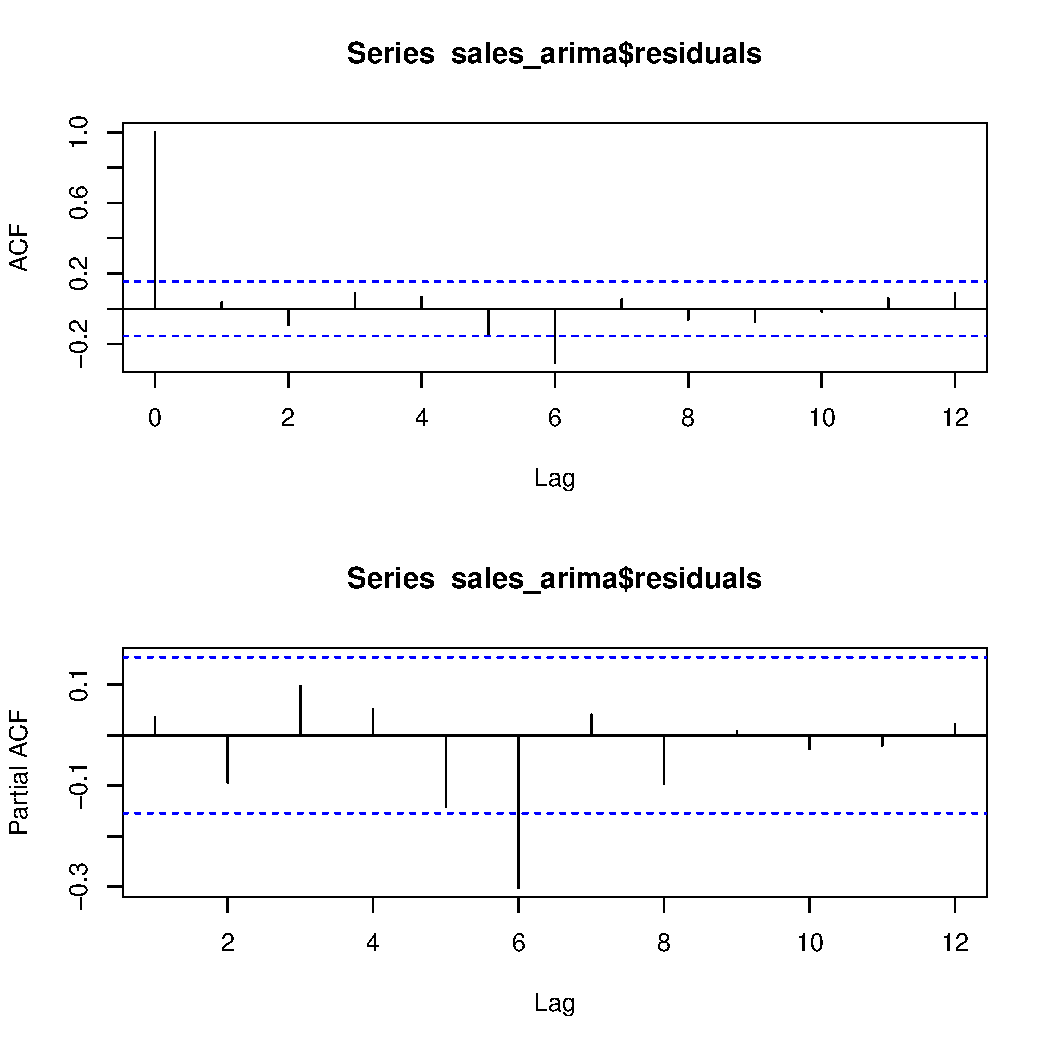
\includegraphics[width=\maxwidth]{figure/unnamed-chunk-6-1} 
\begin{kframe}\begin{alltt}
\hlkwd{par}\hlstd{(}\hlkwc{mfrow} \hlstd{=} \hlkwd{c}\hlstd{(}\hlnum{1}\hlstd{,} \hlnum{1}\hlstd{))}

\hlcom{# Autocorrelation check of residuals}
\hlkwd{Box.test}\hlstd{(sales_arima}\hlopt{$}\hlstd{residuals,} \hlkwc{lag} \hlstd{=} \hlnum{6}\hlstd{,} \hlkwc{type} \hlstd{=} \hlstr{"Ljung"}\hlstd{)}
\end{alltt}
\begin{verbatim}
## 
## 	Box-Ljung test
## 
## data:  sales_arima$residuals
## X-squared = 23.329, df = 6, p-value = 0.0006935
\end{verbatim}
\begin{alltt}
\hlkwd{Box.test}\hlstd{(sales_arima}\hlopt{$}\hlstd{residuals,} \hlkwc{lag} \hlstd{=} \hlnum{12}\hlstd{,} \hlkwc{type} \hlstd{=} \hlstr{"Ljung"}\hlstd{)}
\end{alltt}
\begin{verbatim}
## 
## 	Box-Ljung test
## 
## data:  sales_arima$residuals
## X-squared = 27.461, df = 12, p-value = 0.006628
\end{verbatim}
\end{kframe}
\end{knitrout}

The ACF and PACF both have significant spikes at lag 6 and the Box-Ljung test indicates that there is significant evidence of autocorrelation among the residuals of the time series. Based on this, we will try adding an moving average (MA) term at lag 6 only (not lags 1-6). 

\subsection*{Model 2: ARIMA(2, 1, (6))}

\begin{knitrout}
\definecolor{shadecolor}{rgb}{0.969, 0.969, 0.969}\color{fgcolor}\begin{kframe}
\begin{alltt}
\hlcom{# The "fixed = " term makes it so that the first 5 MA terms are set exactly equal }
\hlcom{# to zero and not evaluated. The default behavior is to fit all MA terms. }
\hlstd{sales_arima_2} \hlkwb{<-} \hlstd{forecast}\hlopt{::}\hlkwd{Arima}\hlstd{(sales_ts,} \hlkwc{order} \hlstd{=} \hlkwd{c}\hlstd{(}\hlnum{2}\hlstd{,} \hlnum{1}\hlstd{,} \hlnum{6}\hlstd{),}
                               \hlkwc{include.drift} \hlstd{=} \hlnum{FALSE}\hlstd{,}
                               \hlkwc{fixed} \hlstd{=} \hlkwd{c}\hlstd{(}\hlnum{NA}\hlstd{,} \hlnum{NA}\hlstd{,} \hlnum{0}\hlstd{,} \hlnum{0}\hlstd{,} \hlnum{0}\hlstd{,} \hlnum{0}\hlstd{,} \hlnum{0}\hlstd{,} \hlnum{NA}\hlstd{))}
\hlkwd{summary}\hlstd{(sales_arima_2)}
\end{alltt}
\begin{verbatim}
## Series: sales_ts 
## ARIMA(2,1,6) 
## 
## Coefficients:
##          ar1      ar2  ma1  ma2  ma3  ma4  ma5      ma6
##       0.5339  -0.2514    0    0    0    0    0  -0.3189
## s.e.  0.0766   0.0779    0    0    0    0    0   0.0765
## 
## sigma^2 estimated as 5.573:  log likelihood=-363.42
## AIC=734.84   AICc=735.1   BIC=747.14
## 
## Training set error measures:
##                     ME     RMSE      MAE      MPE     MAPE     MASE      ACF1
## Training set 0.2158168 2.331114 1.840845 0.256667 3.423964 0.816792 0.0289731
\end{verbatim}
\begin{alltt}
\hlstd{lmtest}\hlopt{::}\hlkwd{coeftest}\hlstd{(sales_arima_2)}
\end{alltt}
\begin{verbatim}
## 
## z test of coefficients:
## 
##      Estimate Std. Error z value  Pr(>|z|)    
## ar1  0.533905   0.076557  6.9739 3.082e-12 ***
## ar2 -0.251374   0.077869 -3.2282  0.001246 ** 
## ma6 -0.318865   0.076519 -4.1672 3.084e-05 ***
## ---
## Signif. codes:  0 '***' 0.001 '**' 0.01 '*' 0.05 '.' 0.1 ' ' 1
\end{verbatim}
\begin{alltt}
\hlcom{# Check to see if the residuals of the time series follow a }
\hlcom{# "white noise" process.}
\hlkwd{par}\hlstd{(}\hlkwc{mfrow} \hlstd{=} \hlkwd{c}\hlstd{(}\hlnum{2}\hlstd{,} \hlnum{1}\hlstd{))}
\hlkwd{acf}\hlstd{(sales_arima_2}\hlopt{$}\hlstd{residuals,} \hlkwc{lag.max} \hlstd{=} \hlnum{12}\hlstd{)}
\hlkwd{pacf}\hlstd{(sales_arima_2}\hlopt{$}\hlstd{residuals,} \hlkwc{lag.max} \hlstd{=} \hlnum{12}\hlstd{)}
\end{alltt}
\end{kframe}
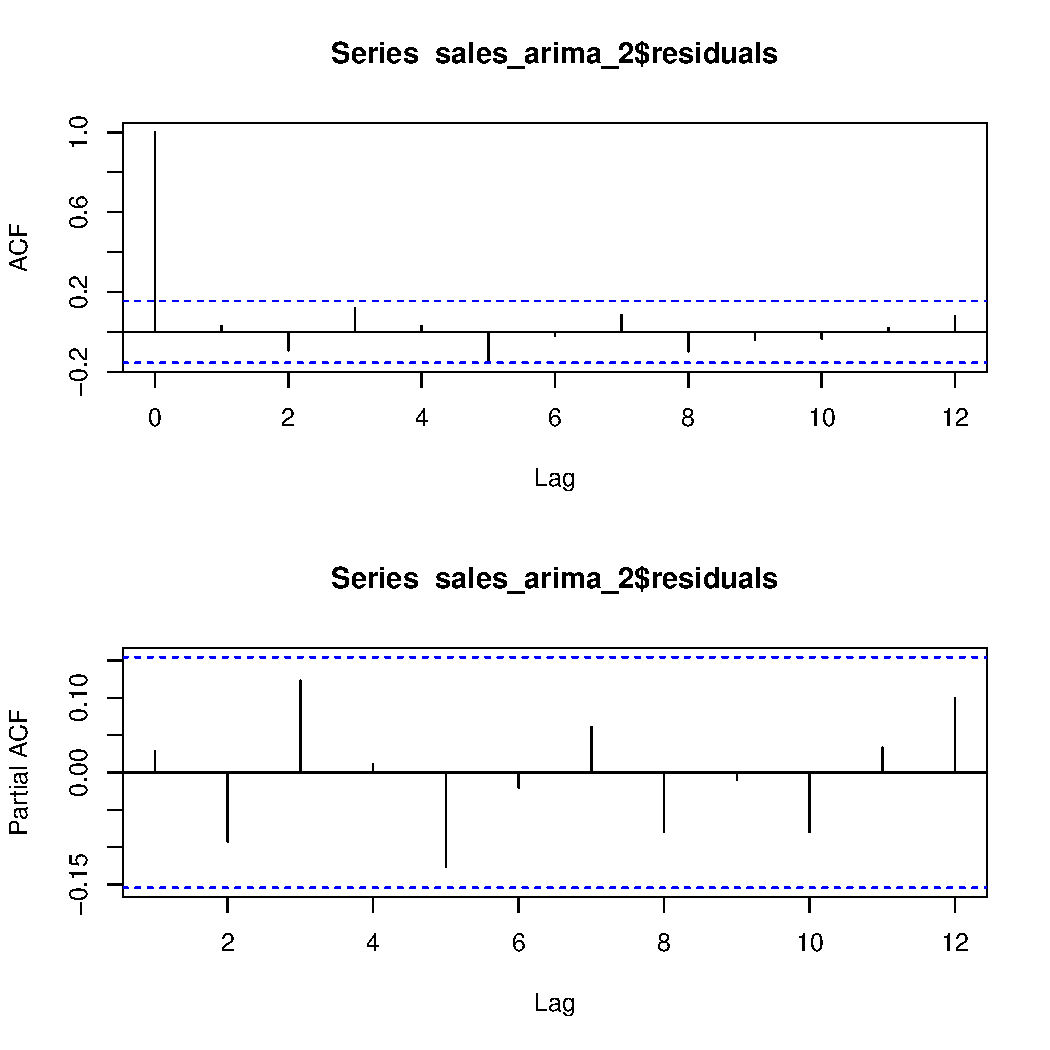
\includegraphics[width=\maxwidth]{figure/unnamed-chunk-7-1} 
\begin{kframe}\begin{alltt}
\hlkwd{par}\hlstd{(}\hlkwc{mfrow} \hlstd{=} \hlkwd{c}\hlstd{(}\hlnum{1}\hlstd{,} \hlnum{1}\hlstd{))}

\hlcom{# Autocorrelation check of residuals}
\hlkwd{Box.test}\hlstd{(sales_arima_2}\hlopt{$}\hlstd{residuals,} \hlkwc{lag} \hlstd{=} \hlnum{6}\hlstd{,} \hlkwc{type} \hlstd{=} \hlstr{"Ljung"}\hlstd{)}
\end{alltt}
\begin{verbatim}
## 
## 	Box-Ljung test
## 
## data:  sales_arima_2$residuals
## X-squared = 7.4574, df = 6, p-value = 0.2806
\end{verbatim}
\begin{alltt}
\hlkwd{Box.test}\hlstd{(sales_arima_2}\hlopt{$}\hlstd{residuals,} \hlkwc{lag} \hlstd{=} \hlnum{12}\hlstd{,} \hlkwc{type} \hlstd{=} \hlstr{"Ljung"}\hlstd{)}
\end{alltt}
\begin{verbatim}
## 
## 	Box-Ljung test
## 
## data:  sales_arima_2$residuals
## X-squared = 11.88, df = 12, p-value = 0.4554
\end{verbatim}
\end{kframe}
\end{knitrout}

The addition of the MA term seems to eliminate the autocorrelation observed among the residuals.

\subsection*{Model 3: ARIMA(0, 1, (1, 6))}

An alternative reading of the ACF/PACF plots may have suggested an MA(1, 6) model (not discussed in class). We explore that fit here and compare it to model 2. 

\begin{knitrout}
\definecolor{shadecolor}{rgb}{0.969, 0.969, 0.969}\color{fgcolor}\begin{kframe}
\begin{alltt}
\hlstd{sales_arima_3} \hlkwb{<-} \hlstd{forecast}\hlopt{::}\hlkwd{Arima}\hlstd{(sales_ts,} \hlkwc{order} \hlstd{=} \hlkwd{c}\hlstd{(}\hlnum{0}\hlstd{,} \hlnum{1}\hlstd{,} \hlnum{6}\hlstd{),}
                               \hlkwc{include.drift} \hlstd{=} \hlnum{FALSE}\hlstd{,}
                               \hlkwc{fixed} \hlstd{=} \hlkwd{c}\hlstd{(}\hlnum{NA}\hlstd{,} \hlnum{0}\hlstd{,} \hlnum{0}\hlstd{,} \hlnum{0}\hlstd{,} \hlnum{0}\hlstd{,} \hlnum{NA}\hlstd{))}
\hlkwd{summary}\hlstd{(sales_arima_3)}
\end{alltt}
\begin{verbatim}
## Series: sales_ts 
## ARIMA(0,1,6) 
## 
## Coefficients:
##          ma1  ma2  ma3  ma4  ma5      ma6
##       0.6471    0    0    0    0  -0.3522
## s.e.  0.0643    0    0    0    0   0.0513
## 
## sigma^2 estimated as 5.029:  log likelihood=-357.33
## AIC=720.66   AICc=720.81   BIC=729.88
## 
## Training set error measures:
##                     ME     RMSE      MAE       MPE     MAPE      MASE
## Training set 0.1694932 2.221447 1.749323 0.2101374 3.262424 0.7761834
##                      ACF1
## Training set -0.007535187
\end{verbatim}
\begin{alltt}
\hlstd{lmtest}\hlopt{::}\hlkwd{coeftest}\hlstd{(sales_arima_3)}
\end{alltt}
\begin{verbatim}
## 
## z test of coefficients:
## 
##      Estimate Std. Error z value  Pr(>|z|)    
## ma1  0.647142   0.064347 10.0571 < 2.2e-16 ***
## ma6 -0.352219   0.051263 -6.8708 6.386e-12 ***
## ---
## Signif. codes:  0 '***' 0.001 '**' 0.01 '*' 0.05 '.' 0.1 ' ' 1
\end{verbatim}
\begin{alltt}
\hlcom{# Check to see if the residuals of the time series follow a }
\hlcom{# "white noise" process.}
\hlkwd{par}\hlstd{(}\hlkwc{mfrow} \hlstd{=} \hlkwd{c}\hlstd{(}\hlnum{2}\hlstd{,} \hlnum{1}\hlstd{))}
\hlkwd{acf}\hlstd{(sales_arima_3}\hlopt{$}\hlstd{residuals,} \hlkwc{lag.max} \hlstd{=} \hlnum{12}\hlstd{)}
\hlkwd{pacf}\hlstd{(sales_arima_3}\hlopt{$}\hlstd{residuals,} \hlkwc{lag.max} \hlstd{=} \hlnum{12}\hlstd{)}
\end{alltt}
\end{kframe}
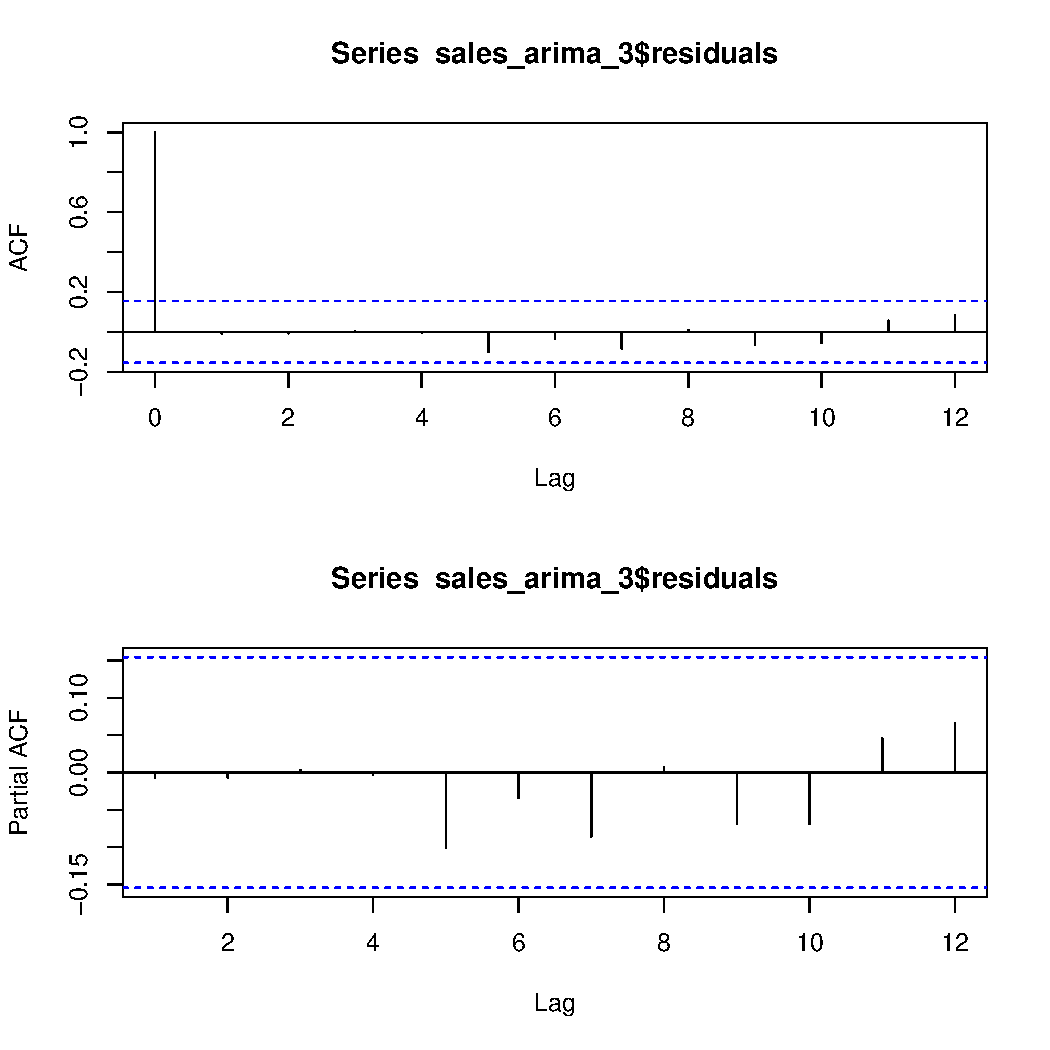
\includegraphics[width=\maxwidth]{figure/unnamed-chunk-8-1} 
\begin{kframe}\begin{alltt}
\hlkwd{par}\hlstd{(}\hlkwc{mfrow} \hlstd{=} \hlkwd{c}\hlstd{(}\hlnum{1}\hlstd{,} \hlnum{1}\hlstd{))}

\hlcom{# Autocorrelation check of residuals}
\hlkwd{Box.test}\hlstd{(sales_arima_3}\hlopt{$}\hlstd{residuals,} \hlkwc{lag} \hlstd{=} \hlnum{6}\hlstd{,} \hlkwc{type} \hlstd{=} \hlstr{"Ljung"}\hlstd{)}
\end{alltt}
\begin{verbatim}
## 
## 	Box-Ljung test
## 
## data:  sales_arima_3$residuals
## X-squared = 1.9065, df = 6, p-value = 0.9281
\end{verbatim}
\begin{alltt}
\hlkwd{Box.test}\hlstd{(sales_arima_3}\hlopt{$}\hlstd{residuals,} \hlkwc{lag} \hlstd{=} \hlnum{12}\hlstd{,} \hlkwc{type} \hlstd{=} \hlstr{"Ljung"}\hlstd{)}
\end{alltt}
\begin{verbatim}
## 
## 	Box-Ljung test
## 
## data:  sales_arima_3$residuals
## X-squared = 6.1106, df = 12, p-value = 0.9104
\end{verbatim}
\end{kframe}
\end{knitrout}

The variance of the residuals in model 3 is slightly less than model 2. Both models 2 and 3 fully account for the spatial autocorrelation in the time series. 

\subsection*{Forecast for Model 2}

\begin{knitrout}
\definecolor{shadecolor}{rgb}{0.969, 0.969, 0.969}\color{fgcolor}\begin{kframe}
\begin{alltt}
\hlstd{ahead_2} \hlkwb{<-} \hlstd{forecast}\hlopt{::}\hlkwd{forecast}\hlstd{(sales_arima_2,} \hlkwc{h} \hlstd{=} \hlnum{25}\hlstd{,} \hlkwc{level} \hlstd{=} \hlnum{95}\hlstd{)}

\hlcom{# 1.96 is the z-score associated with a 95 percent confidence interval}
\hlstd{current} \hlkwb{<-} \hlkwd{data.frame}\hlstd{(}\hlkwc{fit} \hlstd{=} \hlkwd{as.numeric}\hlstd{(sales_arima_2}\hlopt{$}\hlstd{fitted),}
                      \hlkwc{lower} \hlstd{=} \hlkwd{as.numeric}\hlstd{(sales_arima_2}\hlopt{$}\hlstd{fitted} \hlopt{-}
                                           \hlnum{1.96}\hlopt{*}\hlkwd{sqrt}\hlstd{(sales_arima_2}\hlopt{$}\hlstd{sigma2)),}
                      \hlkwc{upper} \hlstd{=} \hlkwd{as.numeric}\hlstd{(sales_arima_2}\hlopt{$}\hlstd{fitted} \hlopt{+}
                                           \hlnum{1.96}\hlopt{*}\hlkwd{sqrt}\hlstd{(sales_arima_2}\hlopt{$}\hlstd{sigma2)),}
                      \hlkwc{week} \hlstd{= sales_df}\hlopt{$}\hlstd{time)}

\hlstd{ahead} \hlkwb{<-} \hlkwd{data.frame}\hlstd{(}\hlkwc{fit} \hlstd{=} \hlkwd{as.numeric}\hlstd{(ahead_2}\hlopt{$}\hlstd{mean),}
                    \hlkwc{lower} \hlstd{=} \hlkwd{as.numeric}\hlstd{(ahead_2}\hlopt{$}\hlstd{lower[,} \hlnum{1}\hlstd{]),}
                    \hlkwc{upper} \hlstd{=} \hlkwd{as.numeric}\hlstd{(ahead_2}\hlopt{$}\hlstd{upper[ ,}\hlnum{1}\hlstd{]),}
                    \hlkwc{week} \hlstd{=} \hlkwd{seq}\hlstd{(}\hlkwd{max}\hlstd{(sales_df}\hlopt{$}\hlstd{time)} \hlopt{+} \hlnum{1}\hlstd{,}
                               \hlkwd{max}\hlstd{(sales_df}\hlopt{$}\hlstd{time)} \hlopt{+} \hlkwd{length}\hlstd{(ahead_2}\hlopt{$}\hlstd{mean)))}

\hlstd{final} \hlkwb{<-} \hlkwd{rbind}\hlstd{(current, ahead)}


\hlkwd{plot}\hlstd{(final}\hlopt{$}\hlstd{week, final}\hlopt{$}\hlstd{fit,} \hlkwc{col} \hlstd{=} \hlstr{"red"}\hlstd{,} \hlkwc{type} \hlstd{=} \hlstr{"l"}\hlstd{,}
     \hlkwc{xlab} \hlstd{=} \hlstr{"week"}\hlstd{,} \hlkwc{ylab} \hlstd{=} \hlstr{"sales"}\hlstd{,}
     \hlkwc{ylim} \hlstd{=} \hlkwd{c}\hlstd{(}\hlnum{0}\hlstd{,} \hlnum{120}\hlstd{),}
     \hlkwc{main} \hlstd{=} \hlstr{"Model Fit: ARIMA(2, 1, (6))"}\hlstd{)}
\hlkwd{lines}\hlstd{(final}\hlopt{$}\hlstd{week, final}\hlopt{$}\hlstd{lower,} \hlkwc{lty} \hlstd{=} \hlnum{2}\hlstd{)}
\hlkwd{lines}\hlstd{(final}\hlopt{$}\hlstd{week, final}\hlopt{$}\hlstd{upper,} \hlkwc{lty} \hlstd{=} \hlnum{2}\hlstd{)}
\hlkwd{lines}\hlstd{(sales_df}\hlopt{$}\hlstd{time, sales_df}\hlopt{$}\hlstd{sales,} \hlkwc{lwd} \hlstd{=} \hlnum{2}\hlstd{,} \hlkwc{col} \hlstd{=} \hlstr{"blue"}\hlstd{)}
\hlkwd{legend}\hlstd{(}\hlstr{"topleft"}\hlstd{,} \hlkwc{legend} \hlstd{=} \hlkwd{c}\hlstd{(}\hlstr{"Observed"}\hlstd{,} \hlstr{"Forecast"}\hlstd{,}
                             \hlstr{"Upper CL (95%)"}\hlstd{,}
                             \hlstr{"Lower CL (95%)"}\hlstd{),}
       \hlkwc{lty} \hlstd{=} \hlkwd{c}\hlstd{(}\hlnum{1}\hlstd{,} \hlnum{1}\hlstd{,} \hlnum{2}\hlstd{,} \hlnum{2}\hlstd{),}
       \hlkwc{col} \hlstd{=} \hlkwd{c}\hlstd{(}\hlstr{"blue"}\hlstd{,} \hlstr{"red"}\hlstd{,} \hlstr{"black"}\hlstd{,} \hlstr{"black"}\hlstd{))}
\end{alltt}
\end{kframe}
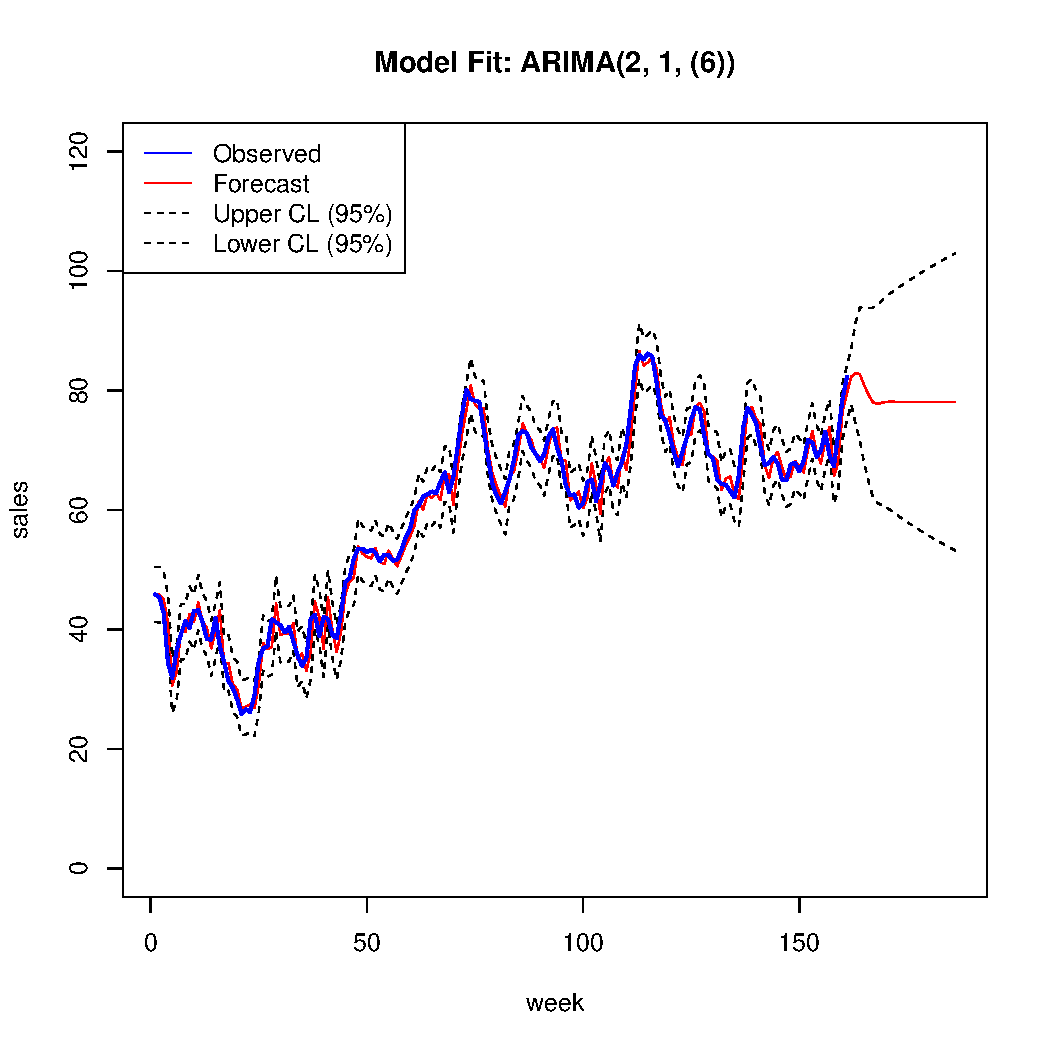
\includegraphics[width=\maxwidth]{figure/unnamed-chunk-9-1} 

\end{knitrout}

\begin{knitrout}
\definecolor{shadecolor}{rgb}{0.969, 0.969, 0.969}\color{fgcolor}\begin{kframe}
\begin{alltt}
\hlstd{ahead_3} \hlkwb{<-} \hlstd{forecast}\hlopt{::}\hlkwd{forecast}\hlstd{(sales_arima_3,} \hlkwc{h} \hlstd{=} \hlnum{25}\hlstd{,} \hlkwc{level} \hlstd{=} \hlnum{95}\hlstd{)}

\hlcom{# 1.96 is the z-score associated with a 95 percent confidence interval}
\hlstd{current} \hlkwb{<-} \hlkwd{data.frame}\hlstd{(}\hlkwc{fit} \hlstd{=} \hlkwd{as.numeric}\hlstd{(sales_arima_3}\hlopt{$}\hlstd{fitted),}
                      \hlkwc{lower} \hlstd{=} \hlkwd{as.numeric}\hlstd{(sales_arima_3}\hlopt{$}\hlstd{fitted} \hlopt{-}
                                           \hlnum{1.96}\hlopt{*}\hlkwd{sqrt}\hlstd{(sales_arima_3}\hlopt{$}\hlstd{sigma2)),}
                      \hlkwc{upper} \hlstd{=} \hlkwd{as.numeric}\hlstd{(sales_arima_3}\hlopt{$}\hlstd{fitted} \hlopt{+}
                                           \hlnum{1.96}\hlopt{*}\hlkwd{sqrt}\hlstd{(sales_arima_3}\hlopt{$}\hlstd{sigma2)),}
                      \hlkwc{week} \hlstd{= sales_df}\hlopt{$}\hlstd{time)}

\hlstd{ahead} \hlkwb{<-} \hlkwd{data.frame}\hlstd{(}\hlkwc{fit} \hlstd{=} \hlkwd{as.numeric}\hlstd{(ahead_3}\hlopt{$}\hlstd{mean),}
                    \hlkwc{lower} \hlstd{=} \hlkwd{as.numeric}\hlstd{(ahead_3}\hlopt{$}\hlstd{lower[,} \hlnum{1}\hlstd{]),}
                    \hlkwc{upper} \hlstd{=} \hlkwd{as.numeric}\hlstd{(ahead_3}\hlopt{$}\hlstd{upper[ ,}\hlnum{1}\hlstd{]),}
                    \hlkwc{week} \hlstd{=} \hlkwd{seq}\hlstd{(}\hlkwd{max}\hlstd{(sales_df}\hlopt{$}\hlstd{time)} \hlopt{+} \hlnum{1}\hlstd{,}
                               \hlkwd{max}\hlstd{(sales_df}\hlopt{$}\hlstd{time)} \hlopt{+} \hlkwd{length}\hlstd{(ahead_3}\hlopt{$}\hlstd{mean)))}

\hlstd{final} \hlkwb{<-} \hlkwd{rbind}\hlstd{(current, ahead)}


\hlkwd{plot}\hlstd{(final}\hlopt{$}\hlstd{week, final}\hlopt{$}\hlstd{fit,} \hlkwc{col} \hlstd{=} \hlstr{"red"}\hlstd{,} \hlkwc{type} \hlstd{=} \hlstr{"l"}\hlstd{,}
     \hlkwc{xlab} \hlstd{=} \hlstr{"week"}\hlstd{,} \hlkwc{ylab} \hlstd{=} \hlstr{"sales"}\hlstd{,}
     \hlkwc{ylim} \hlstd{=} \hlkwd{c}\hlstd{(}\hlnum{0}\hlstd{,} \hlnum{120}\hlstd{),}
     \hlkwc{main} \hlstd{=} \hlstr{"Model Fit: ARIMA(0, 1, (1, 6))"}\hlstd{)}
\hlkwd{lines}\hlstd{(final}\hlopt{$}\hlstd{week, final}\hlopt{$}\hlstd{lower,} \hlkwc{lty} \hlstd{=} \hlnum{2}\hlstd{)}
\hlkwd{lines}\hlstd{(final}\hlopt{$}\hlstd{week, final}\hlopt{$}\hlstd{upper,} \hlkwc{lty} \hlstd{=} \hlnum{2}\hlstd{)}
\hlkwd{lines}\hlstd{(sales_df}\hlopt{$}\hlstd{time, sales_df}\hlopt{$}\hlstd{sales,} \hlkwc{lwd} \hlstd{=} \hlnum{2}\hlstd{,} \hlkwc{col} \hlstd{=} \hlstr{"blue"}\hlstd{)}
\hlkwd{legend}\hlstd{(}\hlstr{"topleft"}\hlstd{,} \hlkwc{legend} \hlstd{=} \hlkwd{c}\hlstd{(}\hlstr{"Observed"}\hlstd{,} \hlstr{"Forecast"}\hlstd{,}
                             \hlstr{"Upper CL (95%)"}\hlstd{,}
                             \hlstr{"Lower CL (95%)"}\hlstd{),}
       \hlkwc{lty} \hlstd{=} \hlkwd{c}\hlstd{(}\hlnum{1}\hlstd{,} \hlnum{1}\hlstd{,} \hlnum{2}\hlstd{,} \hlnum{2}\hlstd{),}
       \hlkwc{col} \hlstd{=} \hlkwd{c}\hlstd{(}\hlstr{"blue"}\hlstd{,} \hlstr{"red"}\hlstd{,} \hlstr{"black"}\hlstd{,} \hlstr{"black"}\hlstd{))}
\end{alltt}
\end{kframe}
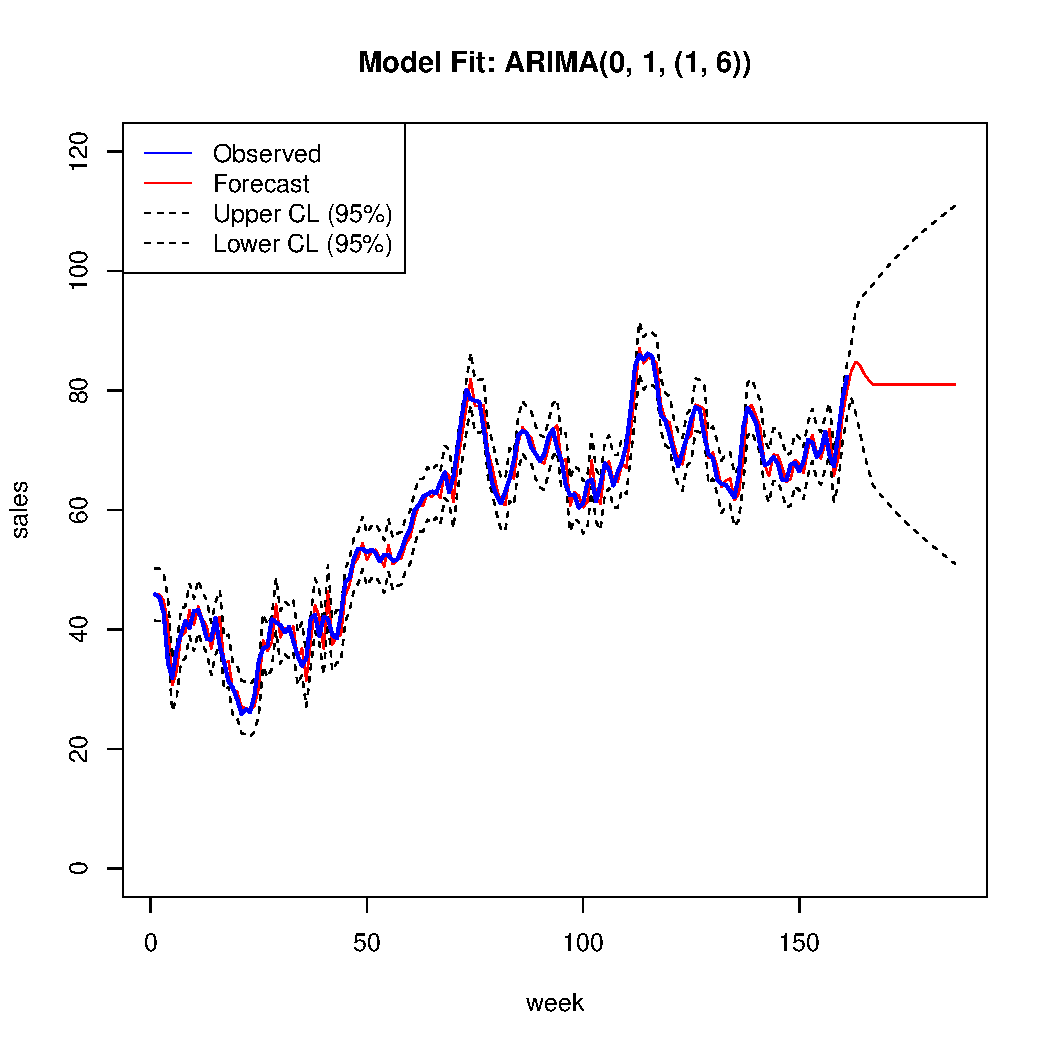
\includegraphics[width=\maxwidth]{figure/unnamed-chunk-10-1} 

\end{knitrout}

Rough Script summarizing these results:

\begin{enumerate}
\item Introduce data and express desire to forecast 25 weeks. \\
\item 
\begin{itemize} 
\item See need for stationarity based on time plot and 
   SAC (p. 2). \\
\item Try linear trend, see remaining ~2 year cycle (p. 3). \\
\item Try linear + trigonometric trends (p. 4). 
   -- But still see problems with 1st-order stationarity. 
\end{itemize} 
\item See stubbornness of time trends (p. 4), and need for 
   differencing; first diff. appears sufficient (pp. 5-6). \\
\item See need for dependence structure after white noise 
   check in first difference (p. 7). \\
\item Model 1: ARIMA(2,1,0), based on mixture of damped 
   exp. decay and sine waves in SAC, and SPAC cuts off 
   after lag 2 -- note may have additional spikes at lags 5 
   and 6 (pp. 8-9). 
   Goodness of fit checks: parameters significant, but 
   model is inadequate (p. 8). \\
\item Model 2: ARIMA(2,1,(6)), based on spike in RSAC of 
   Model 1 (pp. 10-11).
   Goodness of fit checks: no evidence of model 
   inadequacy (pp. 8-9) (? -- note Ljung-Box p-value). \\
\item Model 3: ARIMA(0,1,(1,6)), based on alternative reading 
   of SAC and SPAC of first difference -- on page 7, SAC 
   spikes at lags 1 and 6, SPAC dies down in oscillating 
   fashion.  (pp. 12-13).
   Goodness of fit checks: no evidence of model inadequacy 
   (pp. 12-13). \\
\item Compare forecasts from two 'adequate' models (pp 14-17): 
\begin{itemize}
\item Model 3 better only for short-term (2 week) forecasts, 
     based on tighter confidence intervals (smaller STD for 
     forecasts only for weeks 162-163).
\item Model 2 has tighter confidence intervals (smaller STD)
     for longer-term forecasts (weeks 164-186). 
\end{itemize}
\end{enumerate}


Conclude: 
\begin{itemize}
\item Model 1 inadequate, \\
\item Model 2 best for longer-term forecasts, \\
\item Model 3 best for short-term forecasts 
\end{itemize}

NOTE: One major difference between the R and SAS version of the results is that the R version does not fit an intercept term by default when dealing with differenced data. This can be specified using fit.mean = TRUE (which is the default for un-differenced data). 

\end{document}
